\documentclass{exam}

\usepackage{units} 
\usepackage[fleqn]{amsmath}
\usepackage{float}
\usepackage{mdwlist}
\usepackage{booktabs}
\usepackage{caption}
\usepackage{fullpage}
\usepackage{enumerate}
\usepackage{graphicx}

% \usepackage{2in1, lscape} 

\everymath{\displaystyle}

\author{}
\date{January 22, 2014}
\title{Statistics \\ Week One}

\begin{document}

  \maketitle
  \tableofcontents

  \section{Data}

  \begin{table}[ht]
    \centering
    \begin{tabular}{rlllr}
      \toprule
        ID & Education         & Sex   & Race   & Wages \\
      \midrule
         1 & HS or GED         & Black & Female & 35,000 \\
         2 & HS or GED         & Asian & Female & 30,000 \\
         3 & Master's Degree   & White & Male   & 180,000 \\
         4 & HS or GED         & White & Male   & 92,000 \\
         5 & Some College      & Asian & Female & 80,000 \\
         6 & Some College      & White & Female & 32,000 \\
         7 & Some College      & White & Male   & 65,000 \\
         8 & No HS Diploma     & White & Male   & 22,000 \\
         9 & Bachelor's Degree & White & Male   & 57,000 \\
        10 & Some College      & White & Female & 20,000 \\
      \bottomrule
    \end{tabular}
  \end{table}

  \begin{table}[ht]
    \centering
    \begin{tabular}{rrrrrrrr}
      \toprule
        Std Dev & Min.  & 1st Qu. & Median & Mean  & 3rd Qu. & Max. \\
      \midrule
        48527   & 20000 & 30500   & 46000  & 61300 & 76250   & 180000 \\
      \bottomrule
    \end{tabular}
  \end{table}

  \section{Washington Wages}

  \begin{figure}[H]
    \centering
    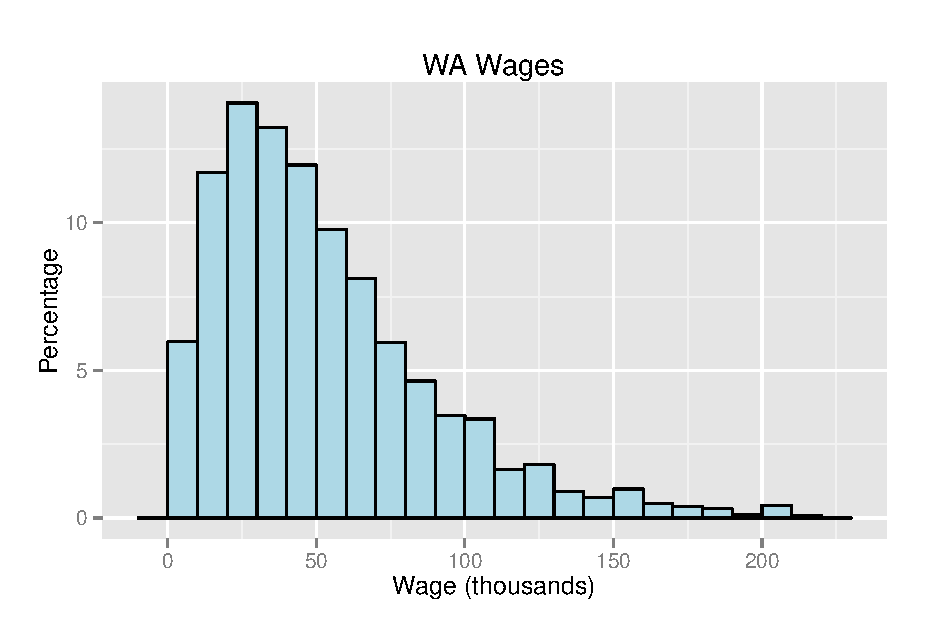
\includegraphics[scale = 0.8]{figures/wa_wage_histogram.eps}
    \caption{WA wage histogram}
  \end{figure}

  \begin{figure}[H]
    \centering
    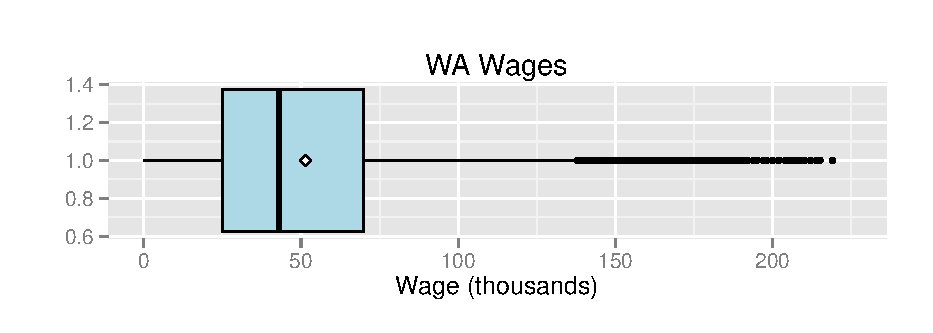
\includegraphics{figures/wa_wage.eps}
    \caption{WA wage box plot}
  \end{figure}

  \begin{table}[ht]
    \centering
    \begin{tabular}{rrrrrrrrr}
      \toprule
        Count & Std Dev & 1st Qu. & Median & Mean  & 3rd Qu. & Max. \\
      \midrule
        24388 & 36689   & 24200   & 42300  & 51240 & 70000   & 219000 \\
      \bottomrule
    \end{tabular}
  \end{table}

  \begin{figure}[H]
    \centering
    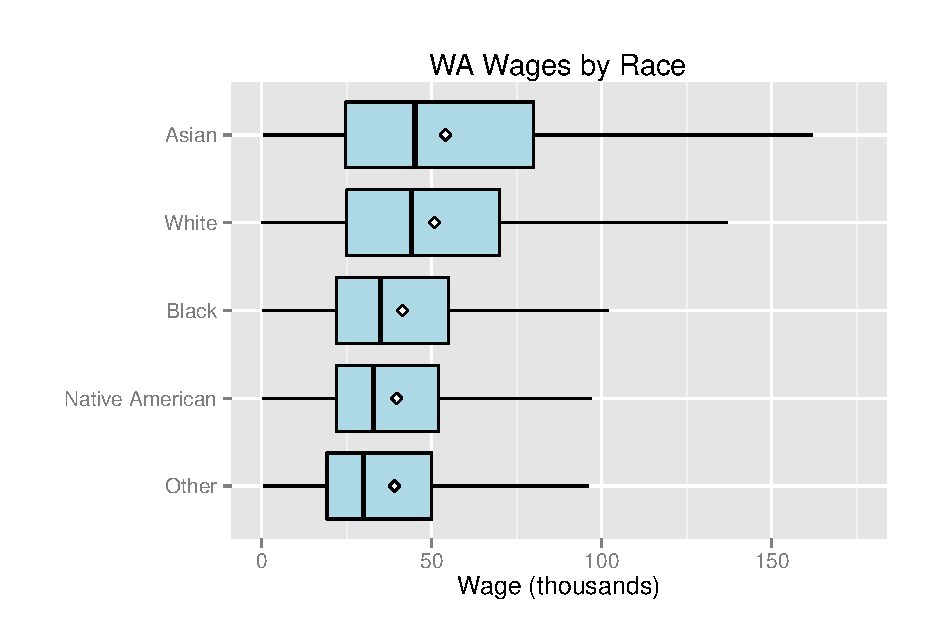
\includegraphics{figures/wa_wage_by_race.eps}
    \caption{WA wages by race}
  \end{figure}

  \begin{table}[ht]
    \centering
    \begin{tabular}{rlrrrrrrrr}
      \toprule
          & race            & Count & Std Dev & Min. & 1st Qu. & Median & Mean  & 3rd Qu. & Max. \\
      \midrule
        1 & Asian           & 1786  & 40247   & 600  & 25000   & 45000  & 55780 & 80000   & 215000 \\
        2 & Black           & 667   & 30004   & 360  & 22000   & 35000  & 41790 & 55000   & 187000 \\
        3 & Native American & 498   & 28512   & 100  & 22000   & 33000  & 40640 & 52750   & 214000 \\
        4 & Other           & 1402  & 31317   & 430  & 19200   & 30000  & 39950 & 50000   & 219000 \\
        5 & White           & 20035 & 36852   & 30   & 25000   & 44900  & 52200 & 70000   & 219000 \\
      \bottomrule
    \end{tabular}
  \end{table}

  \begin{figure}[H]
    \centering
    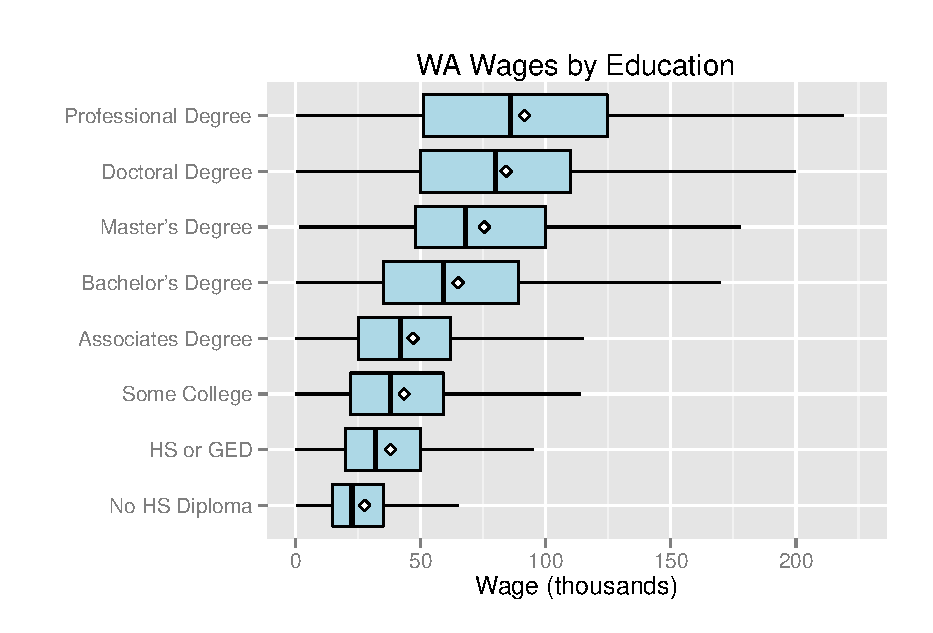
\includegraphics{figures/wa_wage_by_education.eps}
    \caption{WA wages by education}
  \end{figure}

  \begin{table}[ht]
    \centering
    \begin{tabular}{rlrrrrrrrr}
      \toprule
         & education           & Count & Std Dev & Min. & 1st Qu. & Median & Mean  & 3rd Qu. & Max. \\
      \midrule
      1  & Associates Degree   & 2790  & 29158   & 60   & 25000   & 42000  & 46970 & 62000   & 205000 \\
      2  & Bachelor's Degree   & 5687  & 39955   & 380  & 35000   & 59000  & 64930 & 89000   & 215000 \\
      3  & Doctoral Degree     & 368   & 46338   & 200  & 50000   & 80000  & 84110 & 110000  & 212000 \\
      4  & HS or GED           & 5154  & 26030   & 30   & 20000   & 32000  & 37880 & 50000   & 214000 \\
      5  & Master's Degree     & 2230  & 41441   & 1500 & 48000   & 68000  & 75450 & 100000  & 210000 \\
      6  & No HS Diploma       & 1471  & 21308   & 330  & 14850   & 22500  & 27600 & 35000   & 219000 \\
      7  & Professional Degree & 499   & 52328   & 500  & 51000   & 86000  & 91470 & 124500  & 219000 \\
      8  & Some College        & 6189  & 29779   & 100  & 22000   & 38000  & 43400 & 59000   & 215000 \\
      \midrule
    \end{tabular}
  \end{table}

  \begin{figure}[H]
    \centering
    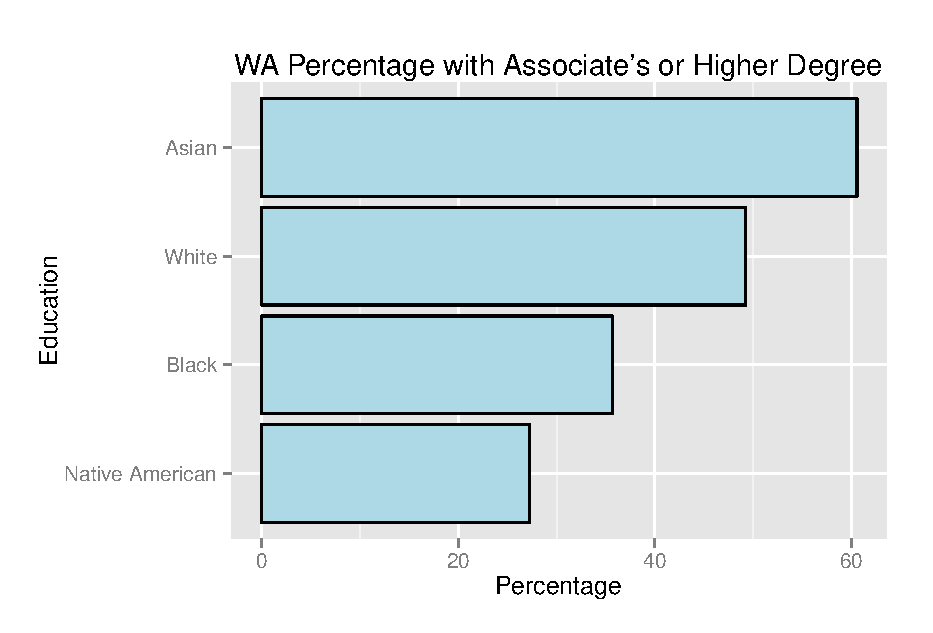
\includegraphics{figures/wa_degree_by_race.eps}
    \caption{Education correlates with wage by race}
  \end{figure}

  \begin{figure}[H]
    \centering
    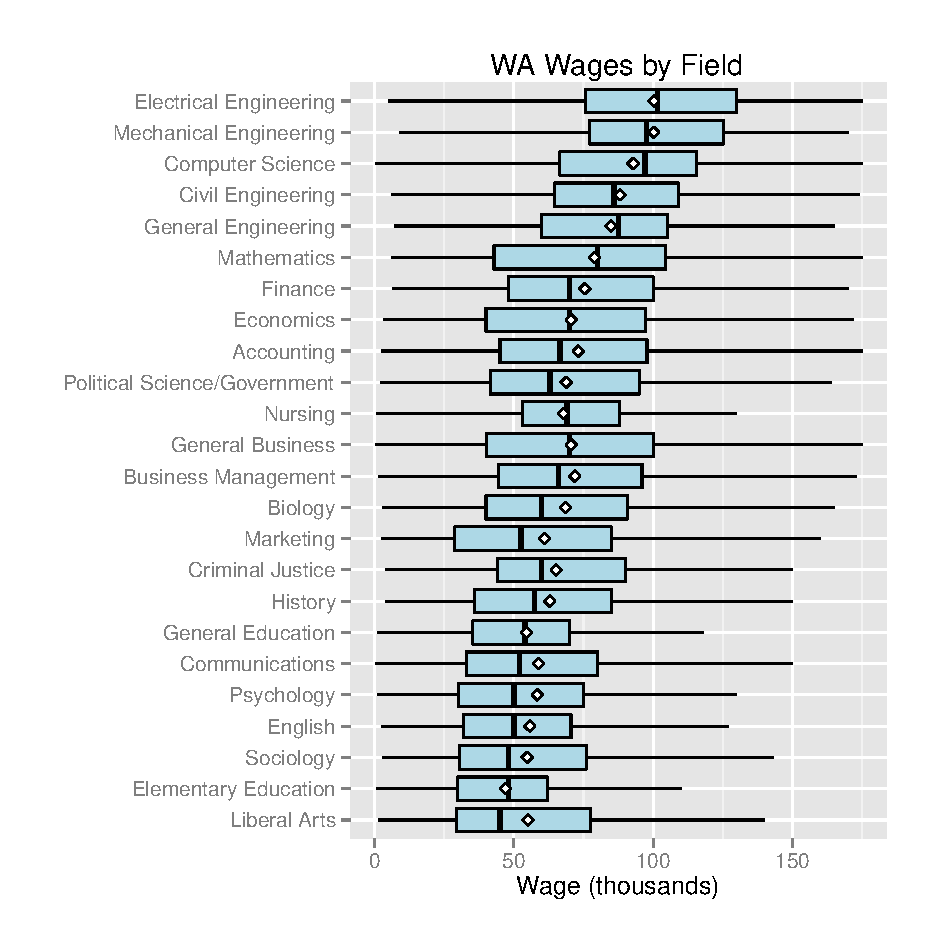
\includegraphics{figures/wa_wage_by_field.eps}
    \caption{WA wages by field}
  \end{figure}

  \begin{table}[ht]
    \centering
    \begin{tabular}{lrrrrrrrr}
      \toprule
      Field                        & Count & Std Dev & Min. & 1st Qu. & Median & Mean   & 3rd Qu. & Max. \\
      \midrule
      Electrical Engineering       & 246   & 43522   & 5000 & 80000   & 104000 & 104000 & 135800  & 207000 \\
      Mechanical Engineering       & 204   & 39081   & 8800 & 78000   & 100000 & 103800 & 130000  & 205000 \\
      Computer Science             & 264   & 43330   & 480  & 70000   & 99500  & 97800  & 120000  & 209000 \\
      Civil Engineering            & 107   & 42577   & 6000 & 65000   & 90000  & 92030  & 115000  & 200000 \\
      General Engineering          & 111   & 43564   & 7000 & 60000   & 90000  & 91620  & 108500  & 200000 \\
      Mathematics                  & 114   & 46415   & 6000 & 45150   & 80000  & 81750  & 108800  & 194000 \\
      Finance                      & 105   & 48302   & 6500 & 48000   & 73000  & 83280  & 108000  & 206000 \\
      Economics                    & 174   & 45074   & 3200 & 42250   & 70000  & 75030  & 100000  & 215000 \\
      General Business             & 293   & 39849   & 400  & 40300   & 70000  & 70580  & 100000  & 175000 \\
      Accounting                   & 254   & 45051   & 2500 & 47250   & 69500  & 77820  & 100000  & 207000 \\
      Nursing                      & 340   & 30967   & 650  & 53000   & 69500  & 68860  & 89000   & 210000 \\
      Business Management          & 545   & 41093   & 1500 & 45000   & 68000  & 74950  & 100000  & 205000 \\
      Political Science/Government & 200   & 41587   & 2000 & 43500   & 65000  & 71390  & 98500   & 208000 \\
      Biology                      & 277   & 48478   & 3000 & 42000   & 64000  & 76270  & 101000  & 219000 \\
      Criminal Justice             & 126   & 34166   & 4000 & 44250   & 60000  & 66260  & 90000   & 200000 \\
      History                      & 179   & 39018   & 4000 & 36500   & 58000  & 65090  & 87500   & 210000 \\
      Marketing                    & 108   & 45394   & 2500 & 29520   & 56000  & 65680  & 85750   & 210000 \\
      General Education            & 227   & 30902   & 1000 & 35650   & 54000  & 55910  & 70000   & 210000 \\
      Communications               & 219   & 40177   & 380  & 33500   & 52000  & 61350  & 80000   & 200000 \\
      English                      & 288   & 34236   & 2600 & 32000   & 50000  & 55710  & 70500   & 175000 \\
      Psychology                   & 394   & 41129   & 1200 & 30180   & 50000  & 60420  & 79750   & 212000 \\
      Sociology                    & 175   & 35710   & 3000 & 30750   & 48200  & 56290  & 78500   & 190000 \\
      Elementary Education         & 204   & 24105   & 600  & 29900   & 48000  & 47010  & 62000   & 120000 \\
      Liberal Arts                 & 153   & 38892   & 1500 & 30000   & 45800  & 57010  & 80000   & 200000 \\
      \bottomrule
    \end{tabular}
  \end{table}

  \begin{figure}[H]
    \centering
    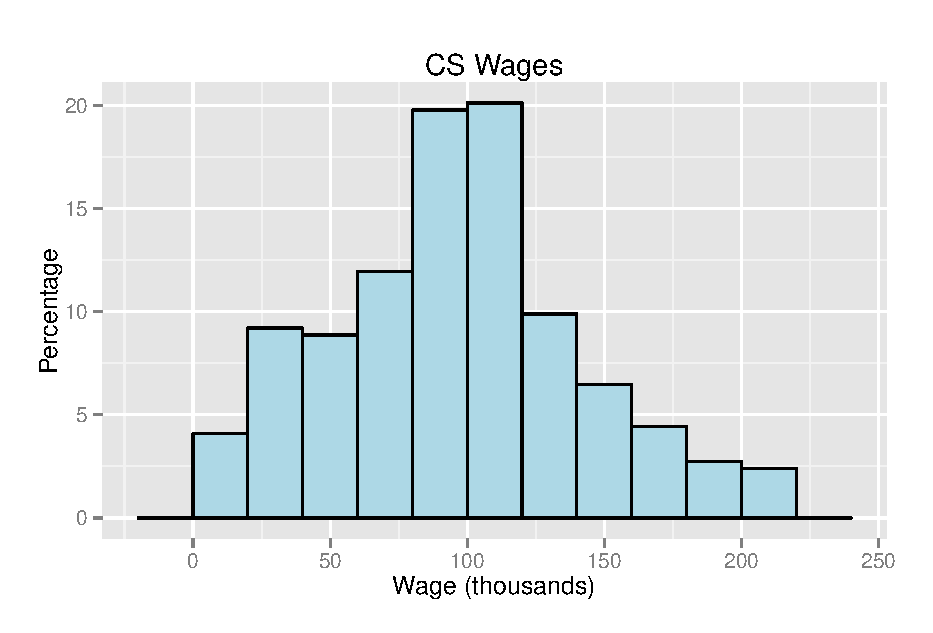
\includegraphics[scale = 0.8]{figures/wa_cs_wages.eps}
    \caption{Computer science wage histogram}
  \end{figure}

  \section{Women vs. Men}

  \begin{figure}[H]
    \centering
    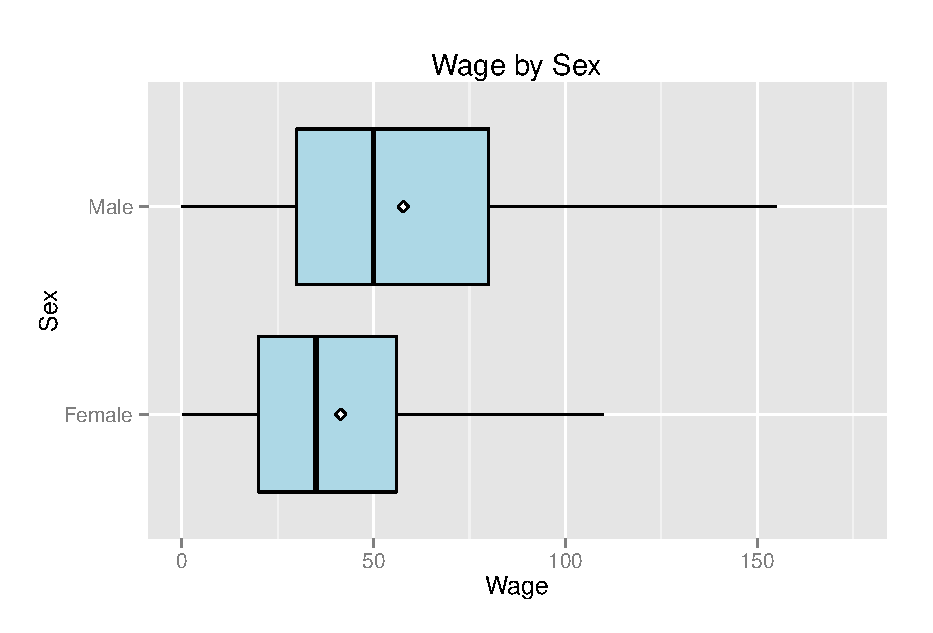
\includegraphics[scale = 0.8]{figures/wa_wage_by_sex.eps}
    \caption{Women make less than men.}
  \end{figure}
  
  \begin{figure}[H]
    \centering
    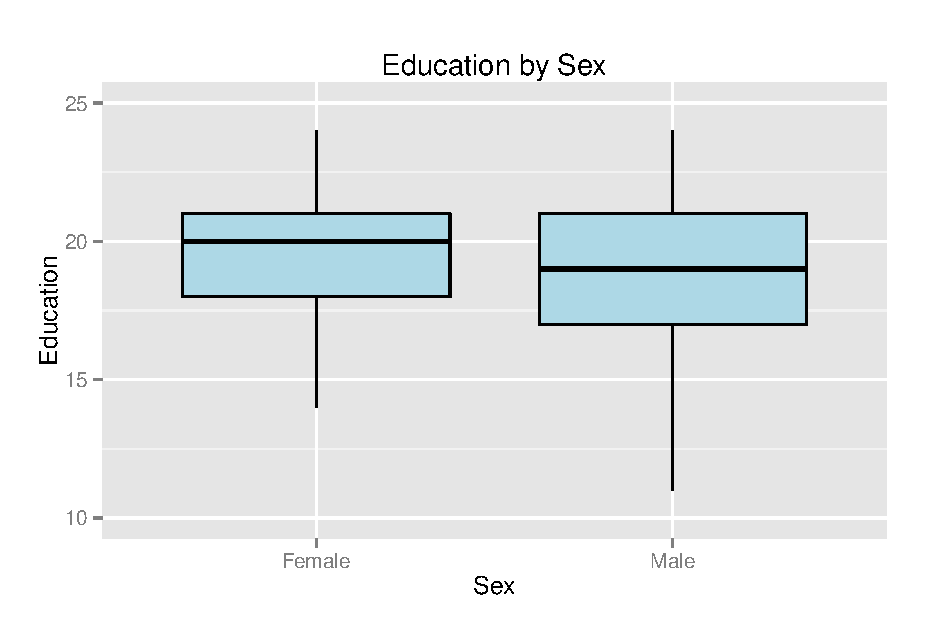
\includegraphics[scale = 0.8]{figures/wa_education_by_sex.eps}
    \caption{Women are a bit more educated than men.}
  \end{figure}

  \begin{figure}[H]
    \centering
    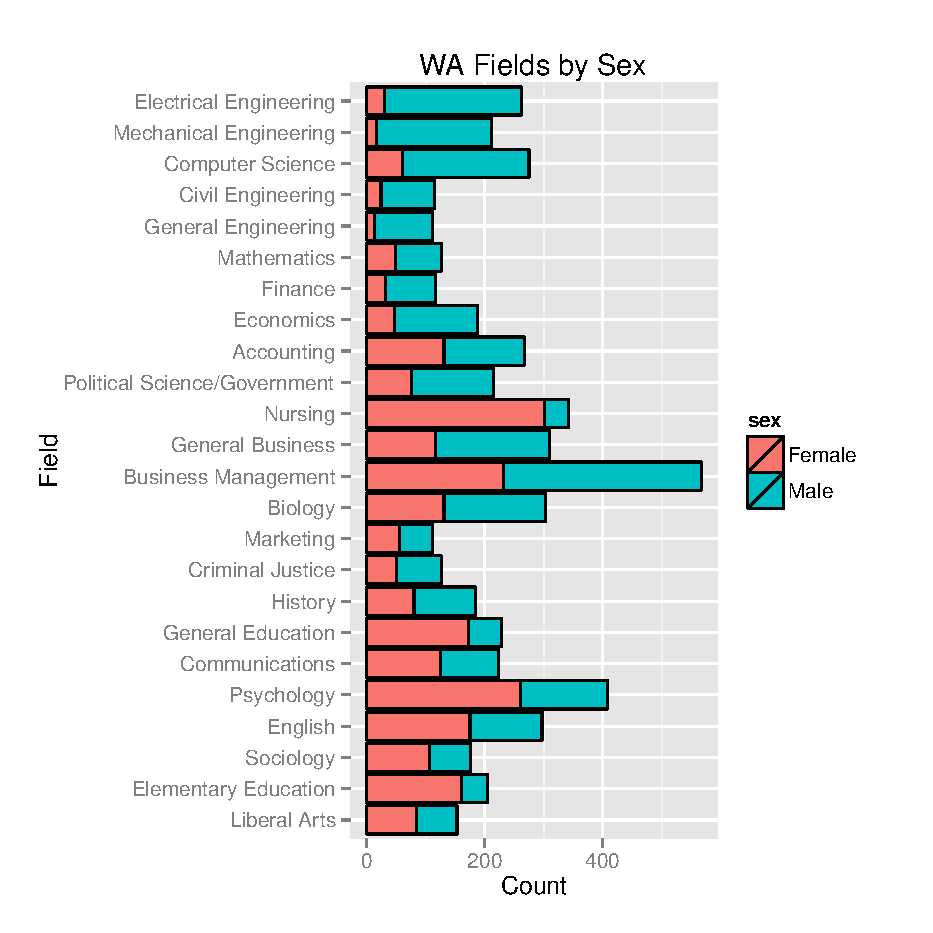
\includegraphics{figures/wa_field_by_sex.eps}
    \caption{ Women tend to get degrees in less lucrative fields.}
  \end{figure}

  
  \begin{figure}[H]
    \centering
    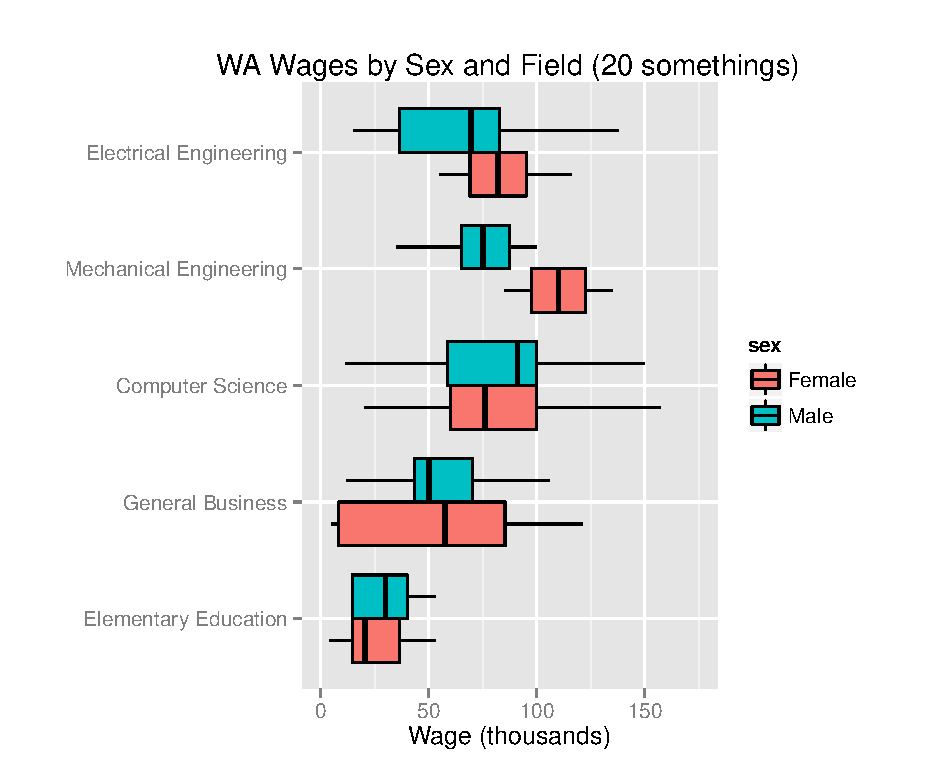
\includegraphics{figures/wa_20s_by_field_and_sex.eps}
    \caption{Twenty to thirty year olds by field seems to be fairly even.}
  \end{figure}

  \begin{figure}[H]
    \centering
    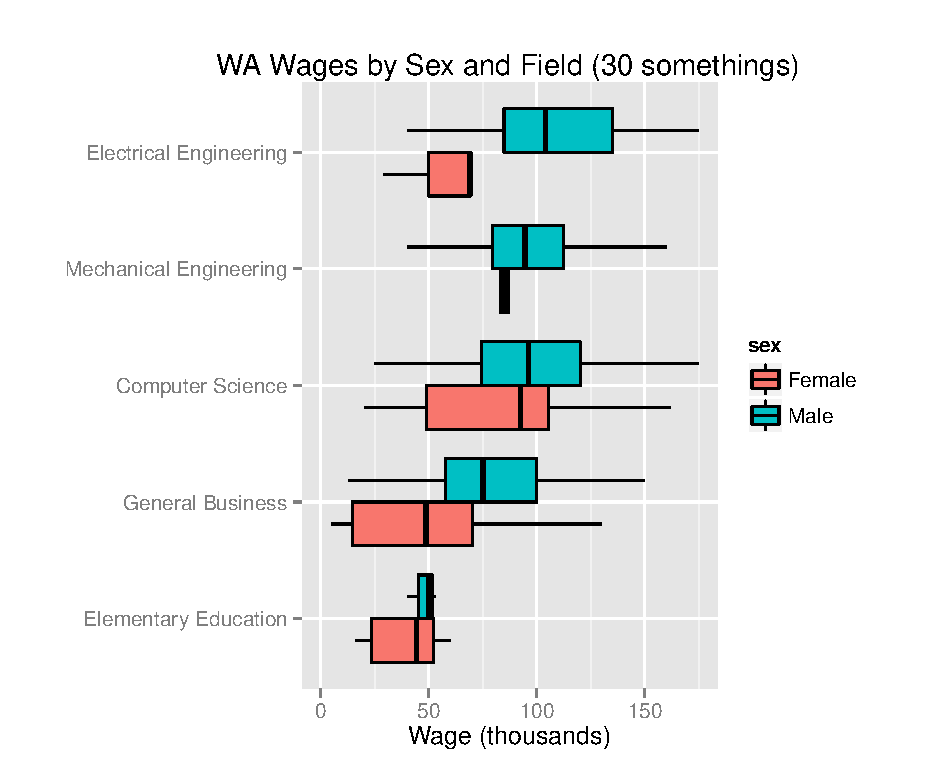
\includegraphics{figures/wa_30s_by_field_and_sex.eps}
    \caption{ Thirty to forty year old men make more than similar women }
  \end{figure}

  \begin{figure}[H]
    \centering
    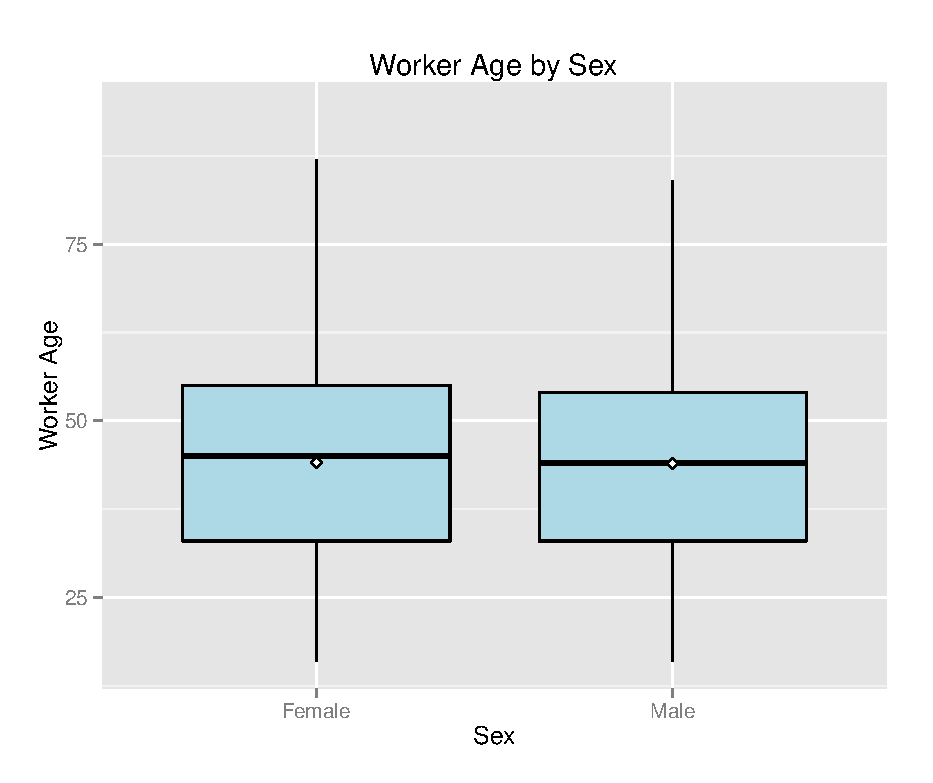
\includegraphics{figures/wa_age_by_sex.eps}
    \caption{Women workers are about the same age as men workers.}
  \end{figure}

  \begin{table}[ht]
    \centering
    \begin{tabular}{rlrrrrrr}
      \toprule
        & sex    & Min. & 1st Qu. & Median & Mean & 3rd Qu. & Max. \\
      \midrule
      1 & Female & 16   & 33      & 45     & 44   & 55      & 94 \\
      2 & Male   & 16   & 33      & 44     & 44   & 54      & 84 \\
      \bottomrule
    \end{tabular}
    \caption{Age by sex}
  \end{table}

  For low education workers, women tend to be older than men.  For high education workers, men tend to be older than
  men.  
  \begin{figure}[H]
    \centering
    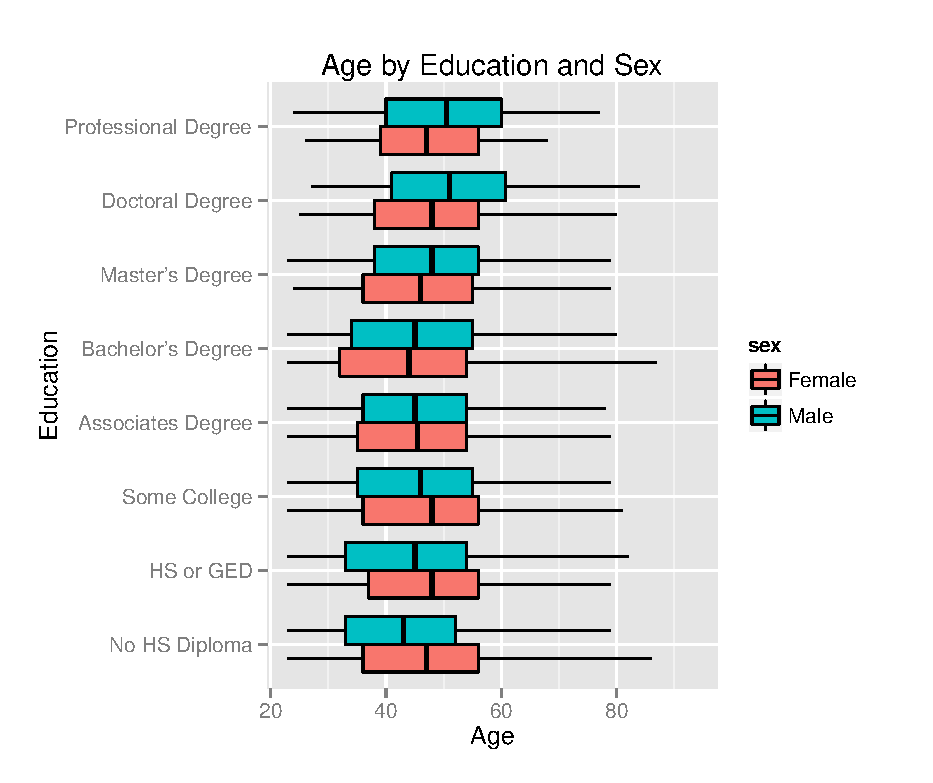
\includegraphics{figures/wa_age_by_education_and_sex.eps}
    \caption{WA wages by education and sex}
  \end{figure}

  \begin{itemize}
    \item men with master's, etc. tend to move up into management. 

    \item women with master's, etc. tend to be married to men with similar education.  They may drop out of the
      workforce when they have kids.  They can afford to do this because of their high income spouses.

    \item women with little education need to work to pay for their kids

    \item women with little education need to work until they are fairly old to survive

  \end{itemize}


\end{document}

